


% \begin{figure}[b]
% \centering

% \begin{minipage}{0.48\linewidth}{
%     % \centering
%     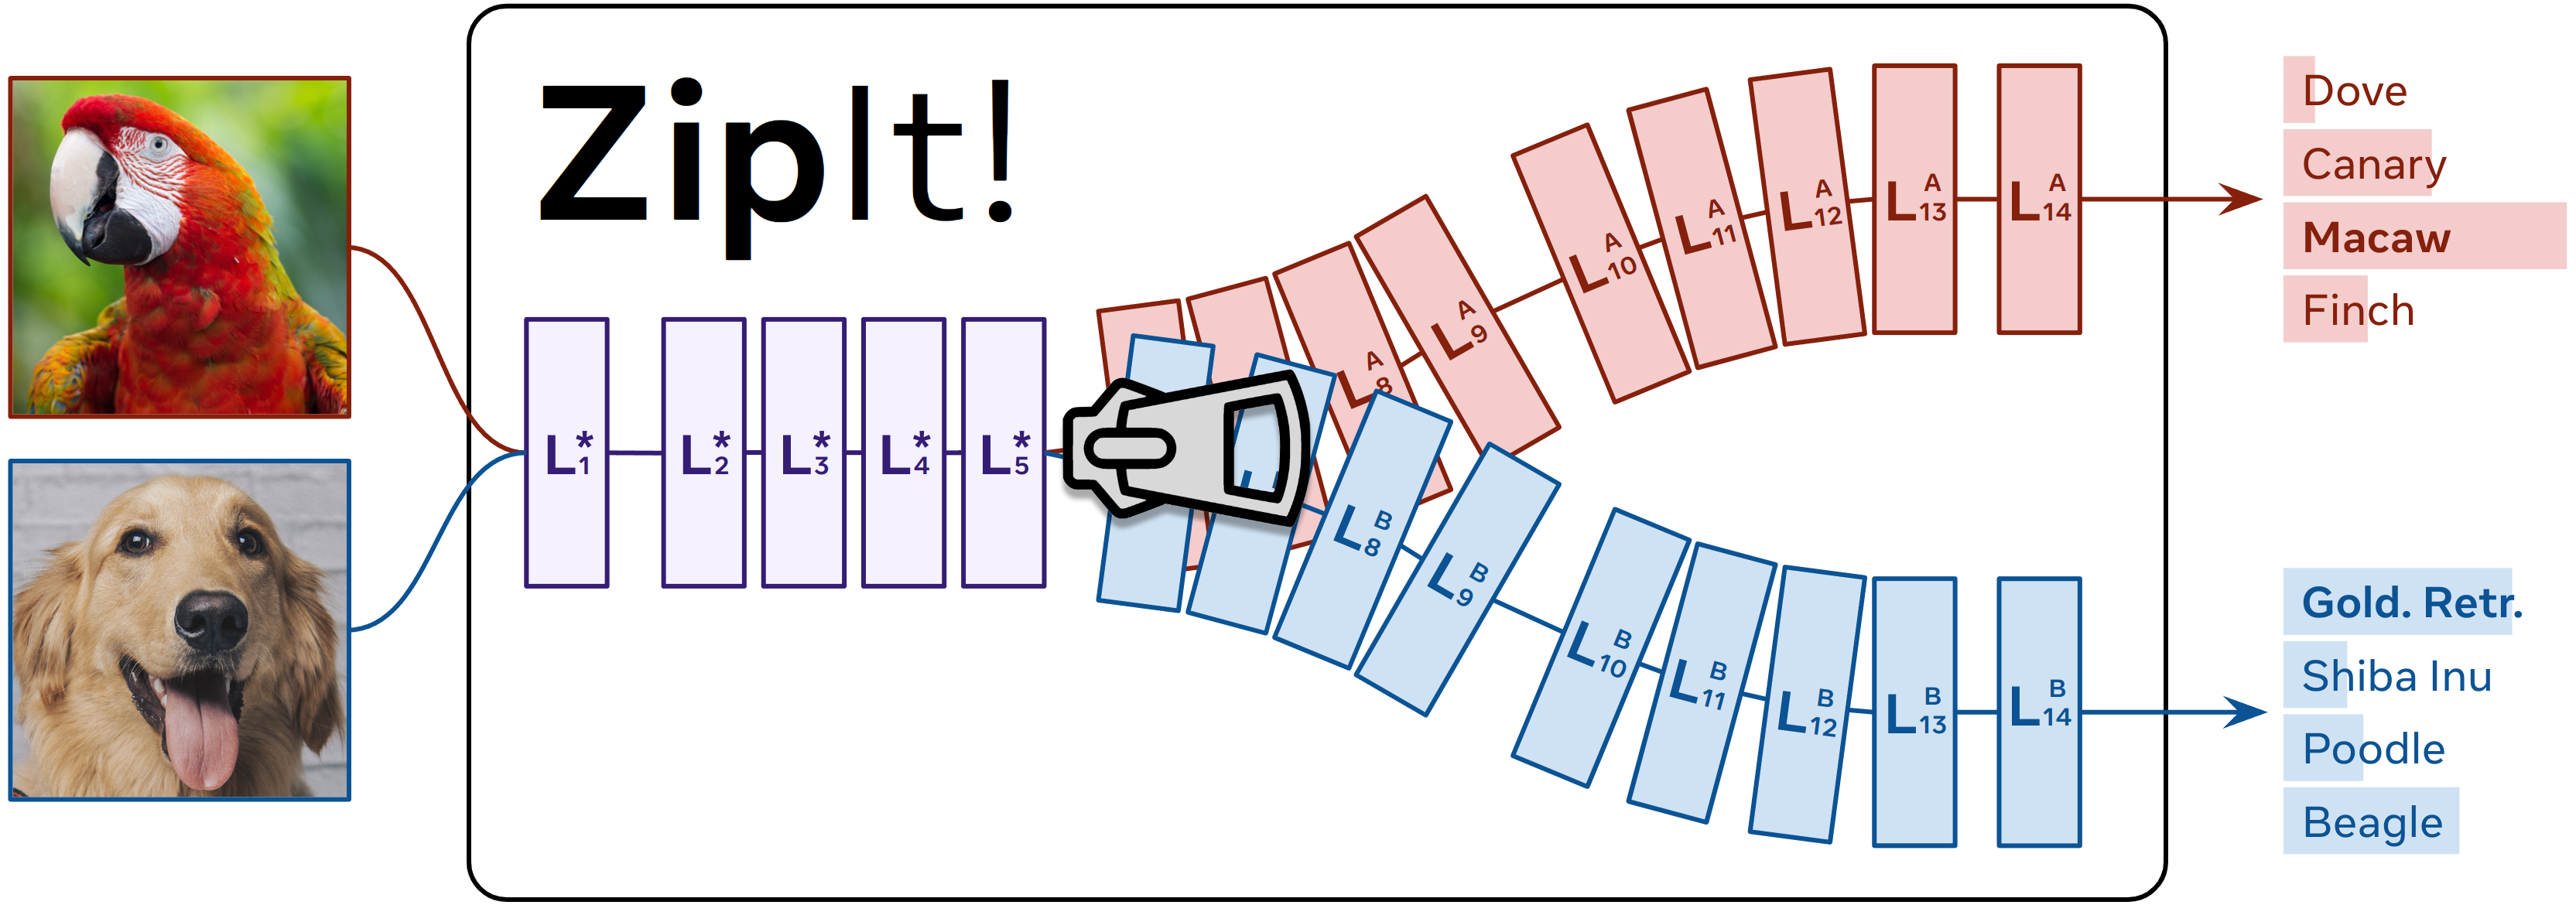
\includegraphics[width=\linewidth]{figures/imgs/concept.png}
%     \caption{{\bf \name{}} merges models trained on completely separate tasks \textit{without any additional training} by identifying their shared features.
%     Depending on the architecture and task, \name{} can nearly match their ensemble performance.
%     }
%     \label{fig:concept}
% }\end{minipage}
% \hspace{1em}
% \begin{minipage}{0.48\linewidth}{
%     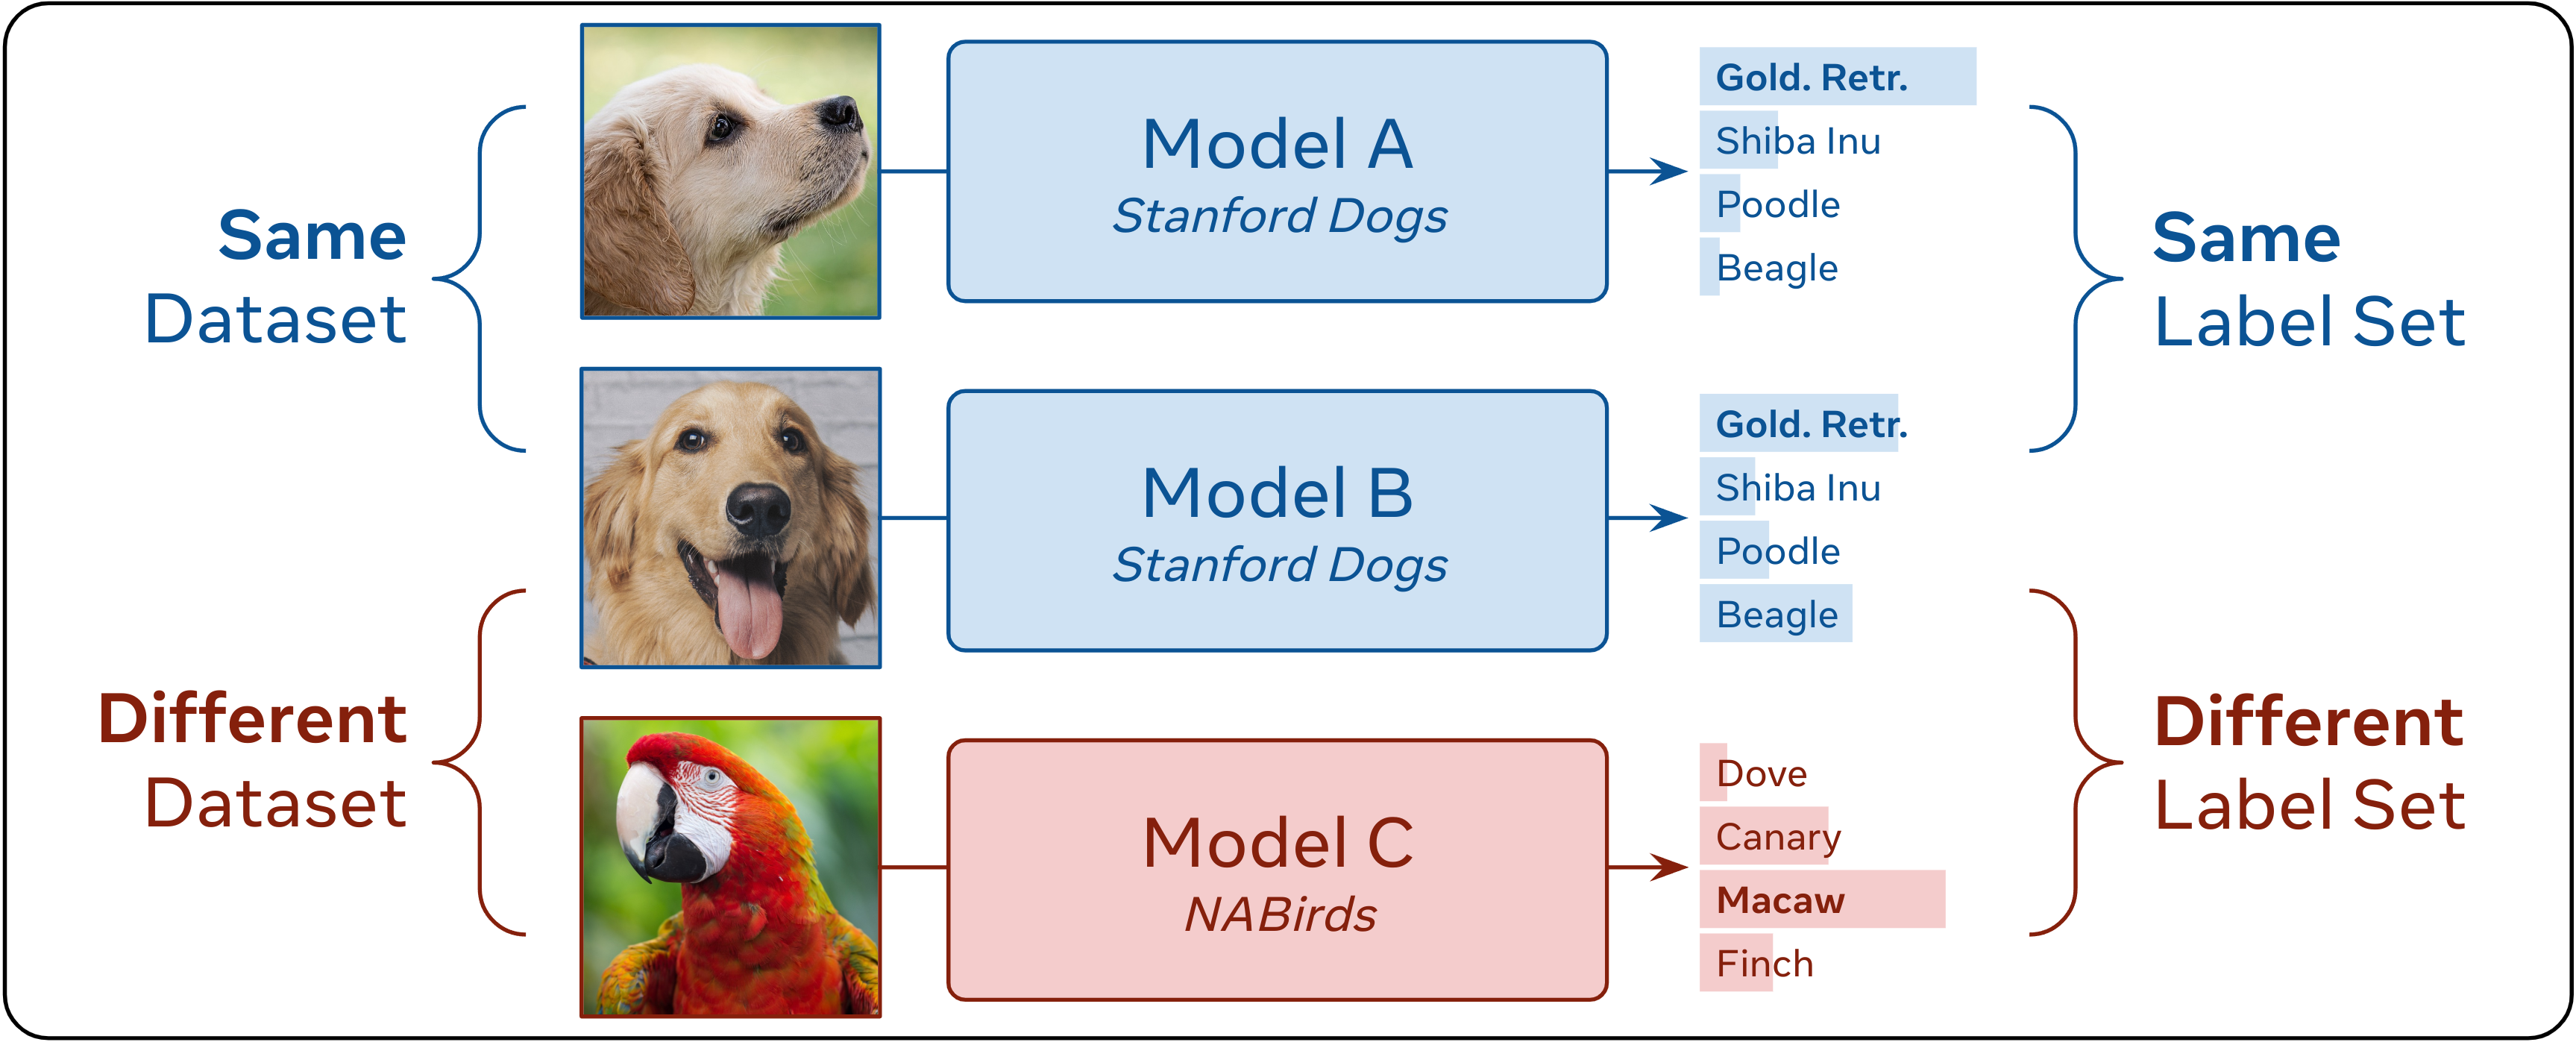
\includegraphics[width=\linewidth]{figures/imgs/vs_prior_work.png}
%     \caption{{\bf Our Setting.} Prior work \cite{wortsman2022model,ainsworth2022git,jordan2022repair}
%     focuses on merging models from the \modelb{\textbf{same} dataset} with the \modelb{\textbf{same} label sets}: e.g., merging two models both trained to classify dog breeds. In this work, we remove that restriction and ``zip'' models that can come from \modela{\textbf{different} datasets} and have \modela{\textbf{different} label sets}: e.g., merging a model that classifies dog breeds with one that classifies bird species.
%     }
%     \label{fig:capabilities}
%     % \includegraphics[width=\linewidth]{figures/imgs/random_r_experiment.png}
    
%     % \captionof{figure}{\textbf{Token Merging Schedule.} Our default constant merging schedule is close to optimal when compared to 15k randomly sampled merging schedules on an AugReg ViT-B/16. }
%     % \label{fig:r_ablation}
% }\end{minipage}
% \end{figure}




\begin{figure}[t]
\centering
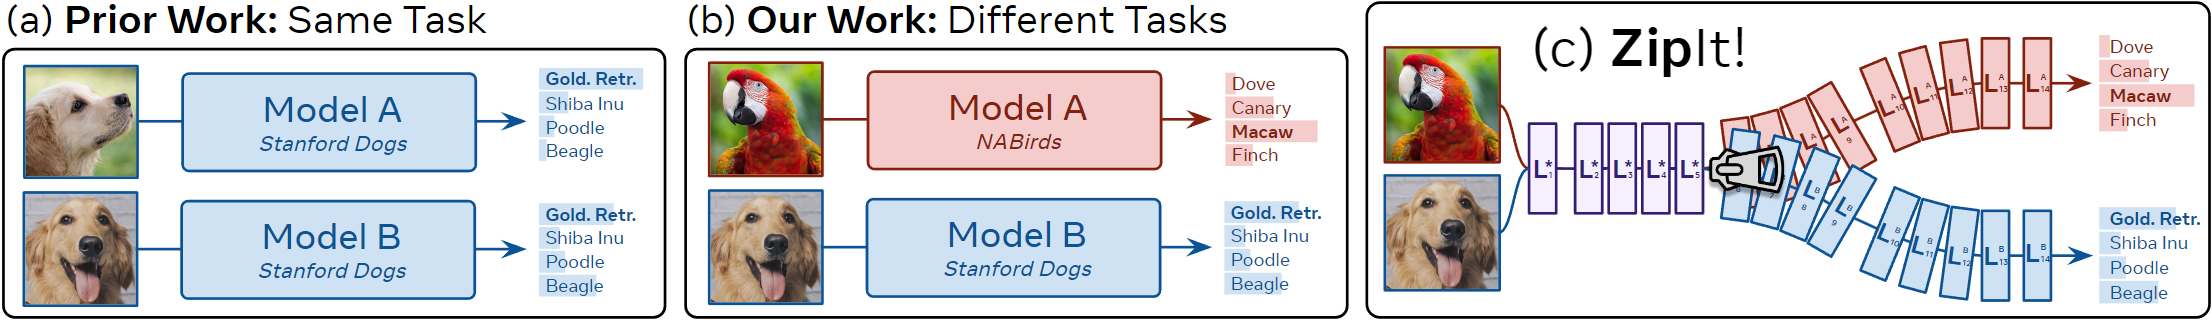
\includegraphics[width=\linewidth]{figures/imgs/concept_and_capabilities.png}
    \caption{
    {\bf Setting and \name{}} (a) Prior work merges differently initialized models from the \modelb{\textbf{same} dataset} with the \modelb{\textbf{same} label sets}: e.g., merging two models both trained to classify dog breeds. (b) Our setting expands this to merging models from \modela{\textbf{different} datasets} with \modela{\textbf{different} label sets}: e.g., merging a model that classifies dog breeds with one that classifies bird species. (c) {\bf \name{}}\ merges these models \textit{without retraining} by identifying shared features.
    }
    \label{fig:concept_and_capabilities}
\end{figure}
